\section{通信系 機能試験(大本)}
通信系の機能試験として行ったのは,以下の4つがある.それぞれについて記述していく.
なお,1,2,3の試験については東京工業大学電気電子系広川研究室の戸村崇助教のご厚意のもと,広川研究室所有の電波暗室をお借りして行った.
\begin{itemize}
	\item モノポールアンテナのインピーダンスマッチング試験
	\item モノポールアンテナの放射特性試験
	\item パッチアンテナの利得・放射特性試験
	\item 長距離通信模擬試験
\end{itemize}

\subsection{通信系設計,機能試験を行うにあたって}
私たち機械系の人間が通信系を担当するのには,かなり大きな専門知識の壁がある.
恐らく利得とは何か,指向性とは何か,偏波とは何か,反射とは何か,周波数が違うと何が変わるのかなど,全く考えたことも無い状態でプロジェクトの通信系を担当することになるだろう.(私もそうだった)
本衛星の開発では,スケジュールの都合などもあり,アンテナ工学などの分野を体系的に学習する時間が取れず,知識の曖昧な状態で機能試験を行い,ほとんど意味のない試験を行ってしまったこともあった.
できるのであれば,簡単な図解の本などでいいからアンテナ工学について体系的な学習を行ってから通信系の開発に臨んでほしい.
「アンテナがわかる本(なるほどナットク!),後藤尚久著,2005年出版」をとりあえず読むことをお勧めする.東工大図書館で借りられる.

\subsection{モノポールアンテナ}
モノポールアンテナには幅5mm,厚さ0.1mmのリン青銅のものを用いた.長さについては後述するインピーダンスマッチング試験から決定した.
リン青銅は錆びる性質があったので,錆びによる性能悪化を防ぐために市販の金メッキキットを用いて金メッキを行った.
「マルイ鍍金工業 めっき工房」というものを購入して利用したが,非常に簡単で使いやすかったのでおすすめ.
図\ref{fig4-7-0}にエンジニアリングモデルのモノポールアンテナを示す.
\begin{figure}[H]
	\centering
	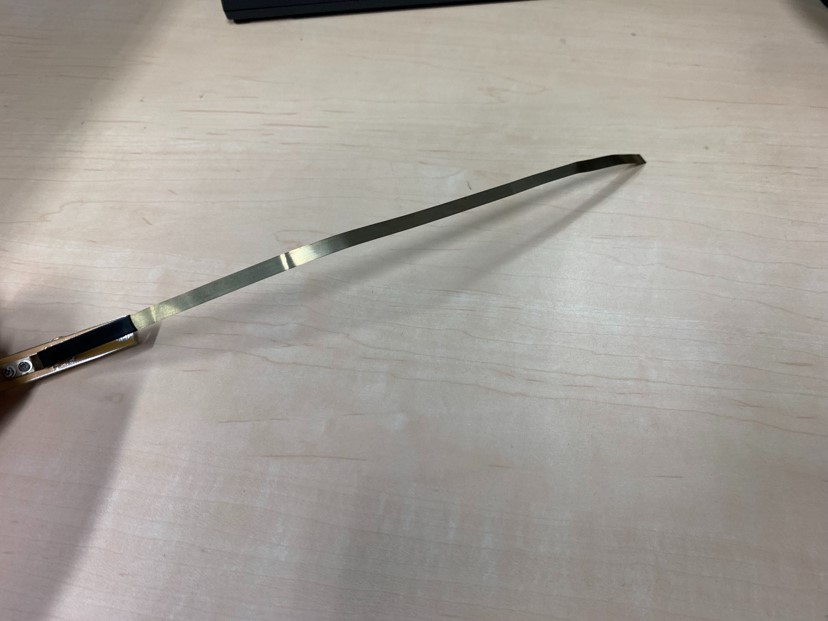
\includegraphics[scale=0.5]{04/fig/4-7-0.jpg}
	\caption{モノポールアンテナ(EM)}
	\label{fig4-7-0}
\end{figure}

\subsection{パッチアンテナ}
パッチアンテナは学生で素子設計を行い,基板製作業者に発注して作成した.
設計に用いた解析ソフトはANSYSのHFSSという電磁界解析ソフト.
専門書などにアンテナ特性の計算ができる式も乗っているが解析ベースで設計しないとまずいいアンテナはできない.
計算式から大まかな寸法の決定→解析によって詳細な寸法の決定という流れ.
特に円偏波で用いる場合,素子寸法は0.1mmのずれで大きく軸比が変化する.
どことは言わないが手加工で円偏波パッチアンテナを作成しているような業者には発注せず,エッチング加工などで製造してくれる業者に発注しよう.
パッチアンテナもモノポールアンテナと同様に錆防止のために金メッキを行った.
図\ref{fig4-7-0-1}にエンジニアリングモデルのパッチアンテナを示す.
\begin{figure}[H]
	\centering
	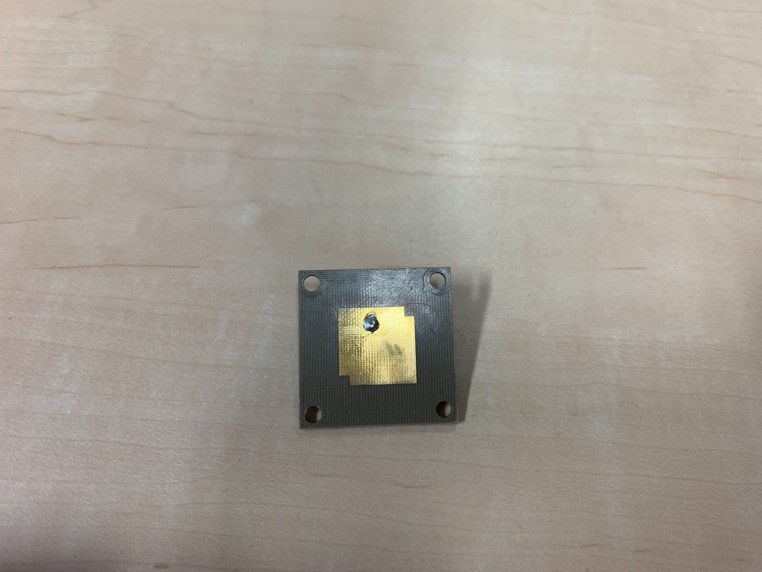
\includegraphics[scale=0.5]{04/fig/4-7-0-1.jpg}
	\caption{パッチアンテナ(EM)}
	\label{fig4-7-0-1}
\end{figure}

\subsection{モノポールアンテナ インピーダンスマッチング試験}
本試験はモノポールアンテナのリターンロスを監視しながらモノポールアンテナの長さを調節することによって,モノポールアンテナの長さを決定するために行った.
インピーダンスマッチング試験の意味については適宜書籍やインターネットなどで調べて理解していただきたい.
試験手順は以下に示す通り.
\begin{enumerate}
	\item モノポールアンテナを取り付けた衛星を電波暗室計測冶具に固定\par
	\quad 電波の放射方向への金属材料などは電波を反射しリターンロスとして計測結果に表れてしまうので,絶縁体を使用する.アクリルプレートや3Dプリンターなどで作成.
	\item VNAを校正し,モノポールアンテナに接続\par
	\quad VNAはネットワークアナライザのこと.ネットワークアナライザは計測するたびに校正が必要であり,また非常に高価な機材のため,宇宙研などどこかの機関に借りる必要あり.本衛星の計測では東工大電気電子系広川研究室の設備をお借りした.
	\item モノポールアンテナをニッパーなどで短く切断していき,長さ対リターンロスの関係を計測\par
	\quad ここで切断するモノポールアンテナはFMとして用いるものではないので,どんどん短くしていく.モノポールアンテナを短くしていくとリターンロスが最小となる周波数は大きくなっていくはずなので,その関係を得ることが目的.図\ref{fig4-7-1},図\ref{fig4-7-1-2}に本衛星の計測結果を示す.
	\begin{figure}[H]
		\centering
		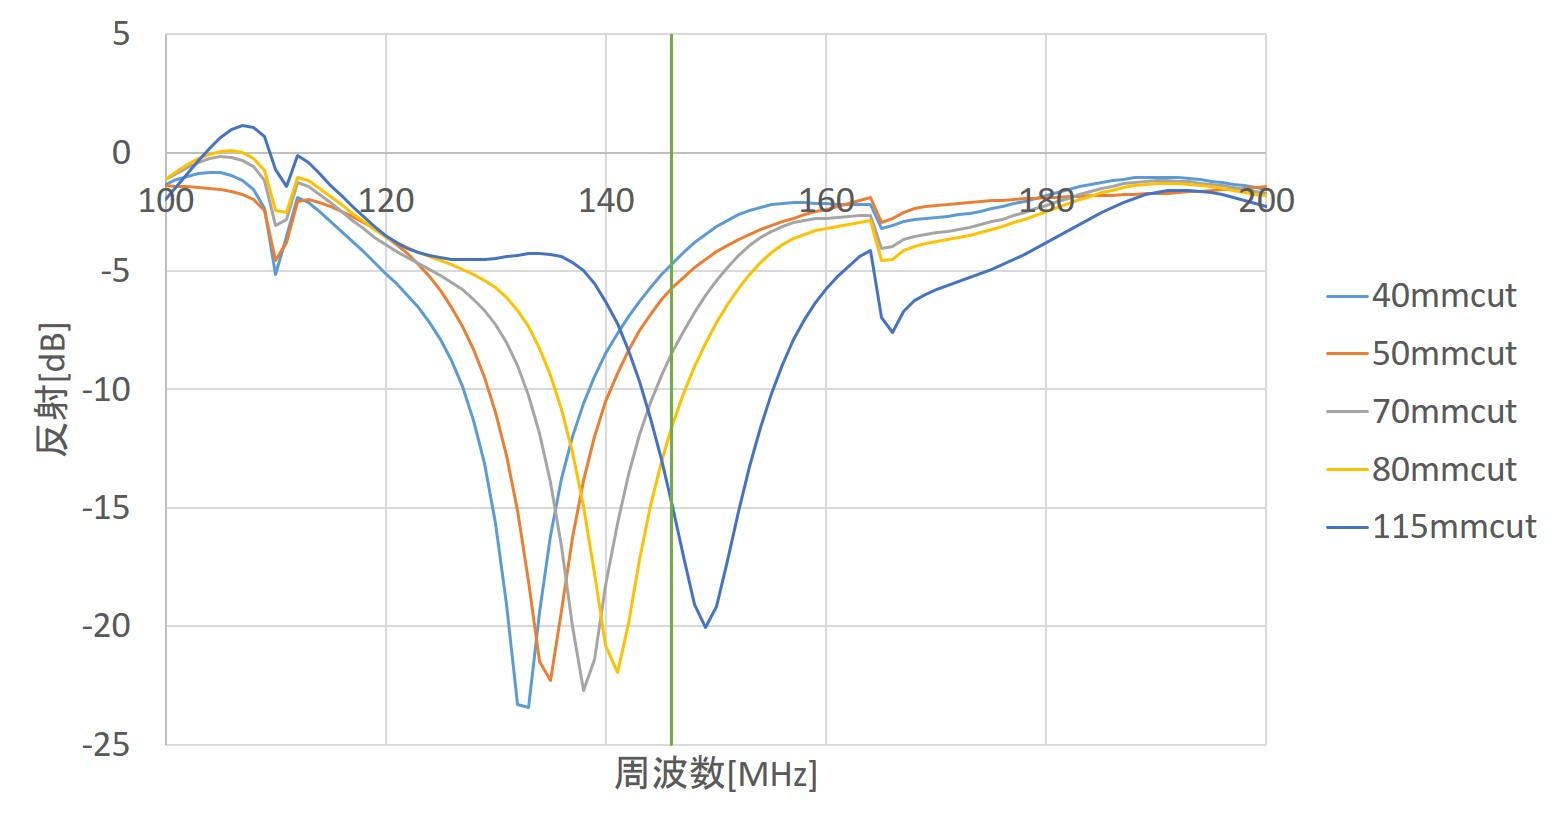
\includegraphics[scale=0.5]{04/fig/4-7-1.jpg}
		\caption{反射対周波数(VHF)}
		\label{fig4-7-1}
	\end{figure}
	\begin{figure}[H]
		\centering
		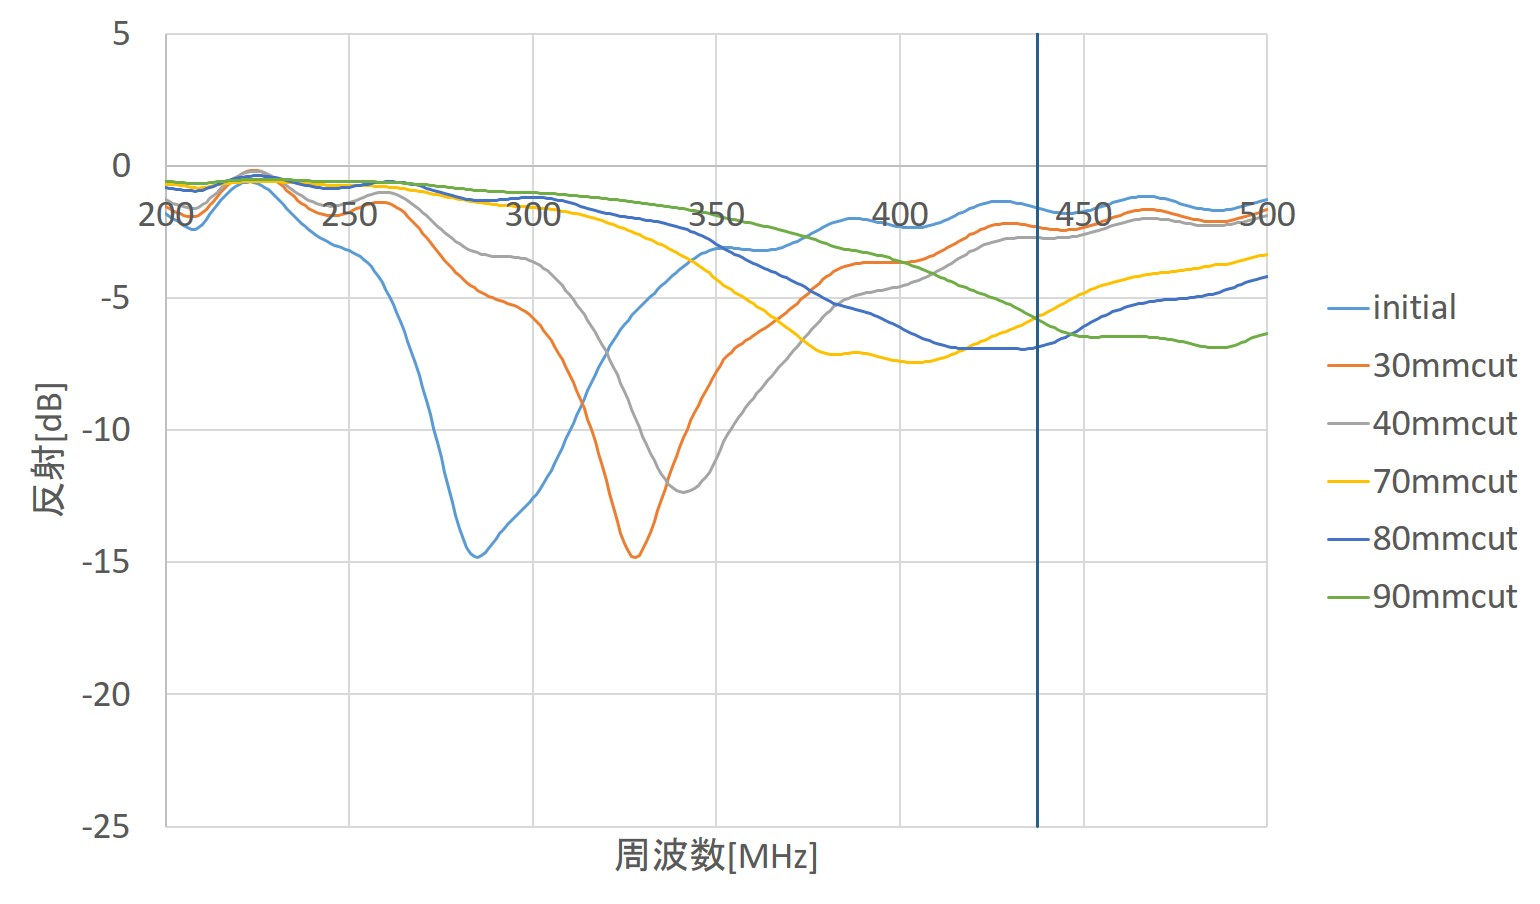
\includegraphics[scale=0.5]{04/fig/4-7-1-2.jpg}
		\caption{反射対周波数(UHF)}
		\label{fig4-7-1-2}
	\end{figure}
	\item 線形近似などを用いて,リターンロスが目標周波数で最小となるようなモノポールアンテナの長さを計算\par
	\quad 得られたリターンロスが最小となる周波数とモノポールアンテナの長さの関係から適当な近似で目標周波数で最小となるモノポールアンテナの長さを決定する.同じ材料で同じように取り付けられたモノポールアンテナは少なくてもMHz帯程度の周波数では同じような特性が得られる.図
	\begin{figure}[H]
		\centering
		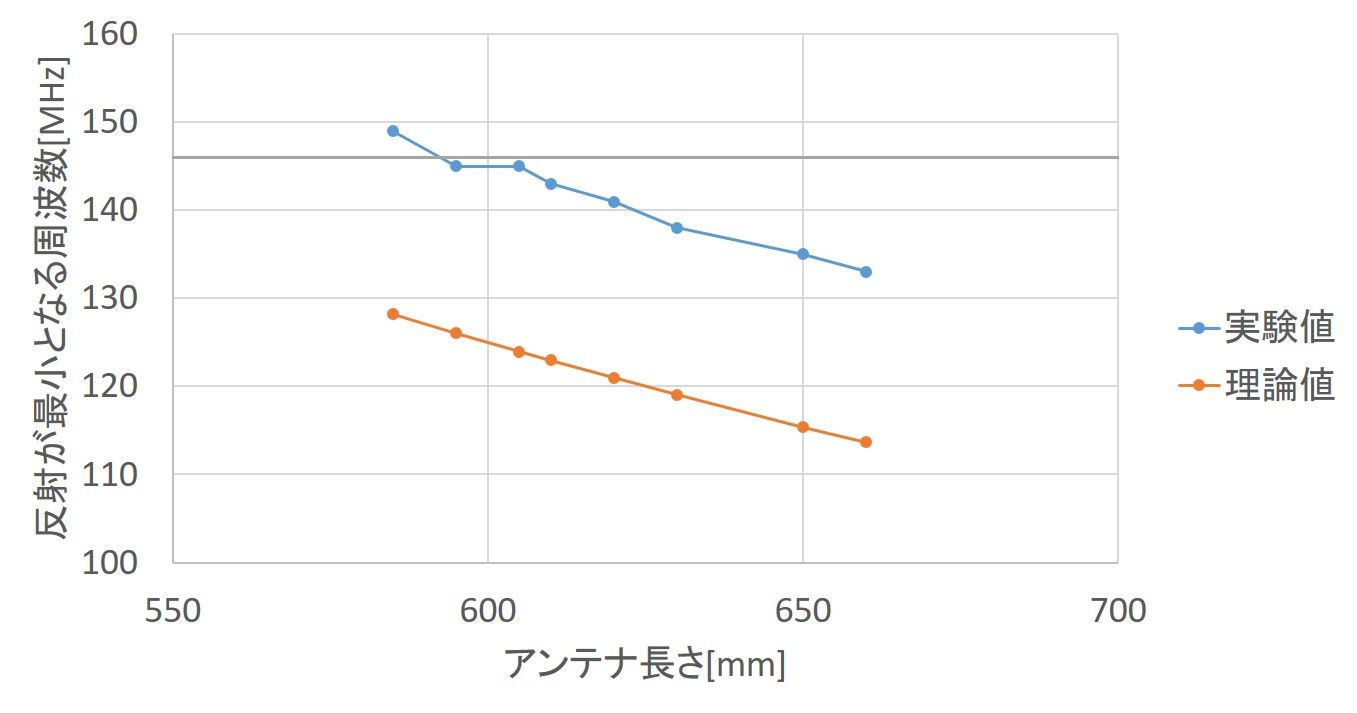
\includegraphics[scale=0.5]{04/fig/4-7-2.jpg}
		\caption{アンテナ長さとリターンロスが最小となる周波数の関係(VHF)}
		\label{fig4-7-2}
	\end{figure}
	\begin{figure}[H]
		\centering
		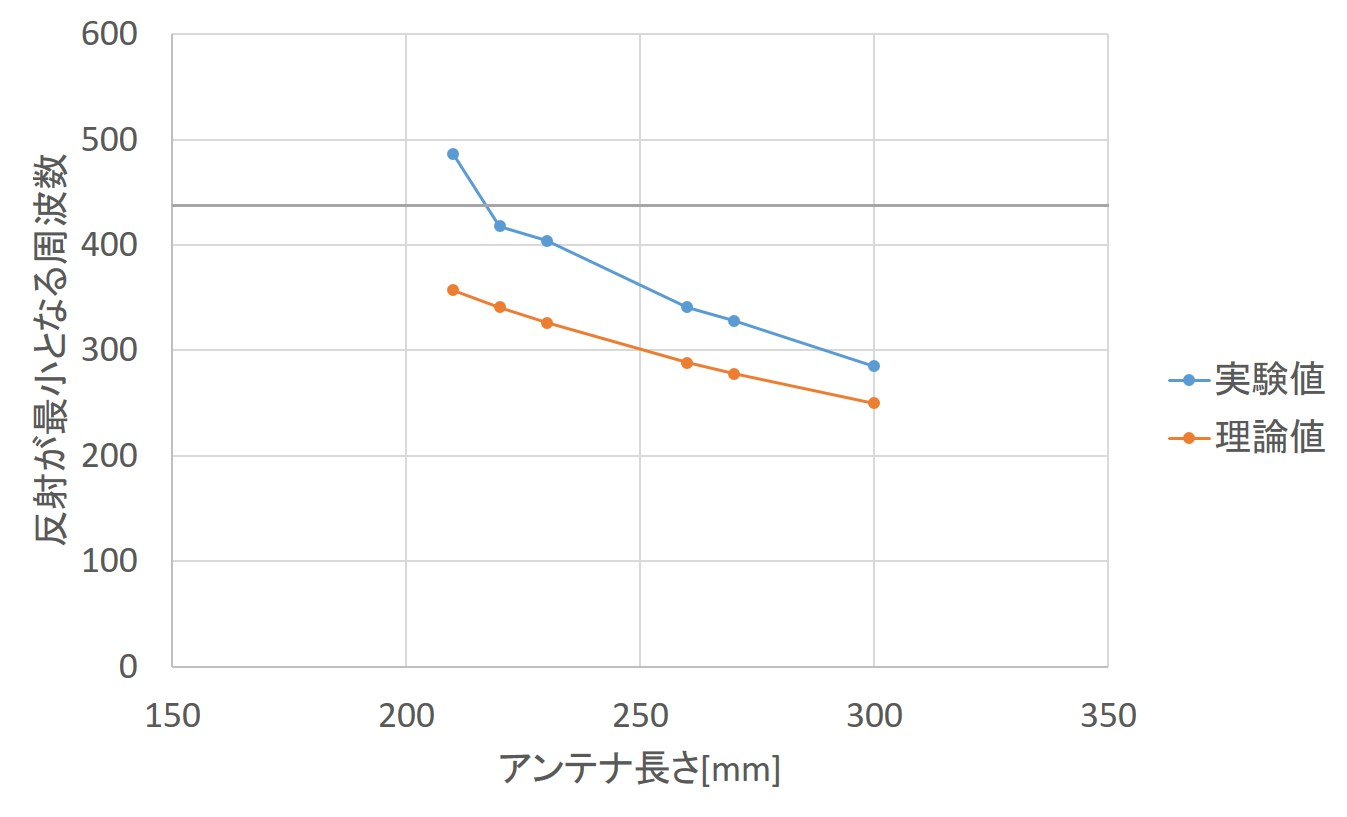
\includegraphics[scale=0.5]{04/fig/4-7-2-2.jpg}
		\caption{アンテナ長さとリターンロスが最小となる周波数の関係(UHF)}
		\label{fig4-7-2-2}
	\end{figure}
	\item 計算した長さのモノポールアンテナを作成し,再度電波暗室でリターンロスを計測\par
	\quad FMとして用いるアンテナの反射特性を計測.図\ref{fig4-7-3}-\ref{fig4-7-3-2}に計測結果を示す.
	\begin{figure}[H]
		\centering
		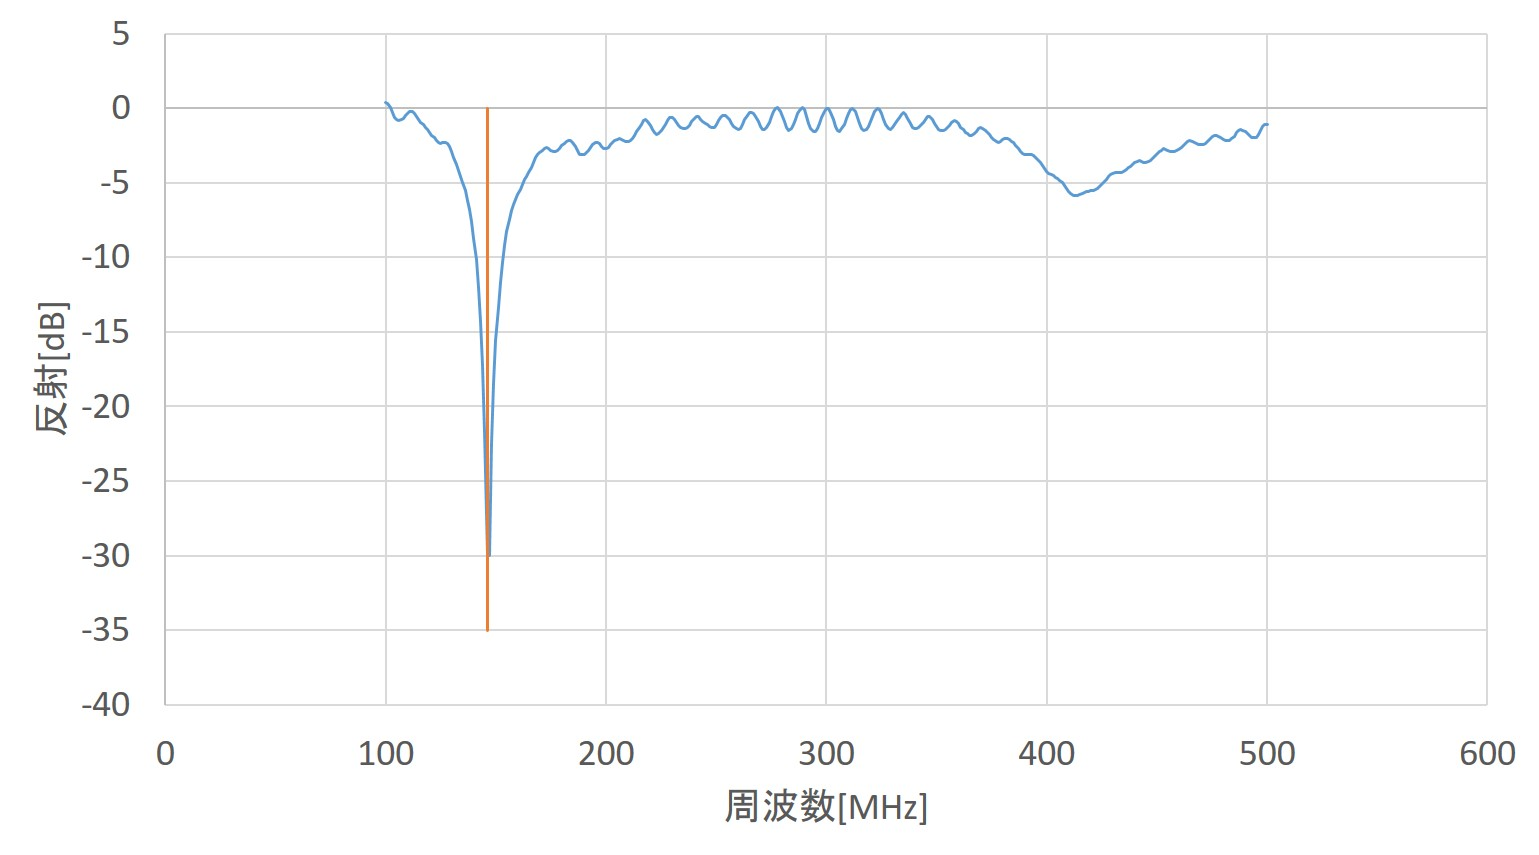
\includegraphics[scale=0.5]{04/fig/4-7-3.jpg}
		\caption{FMモノポールアンテナ反射計測結果(VHF)}
		\label{fig4-7-3}
	\end{figure}
	\begin{figure}[H]
		\centering
		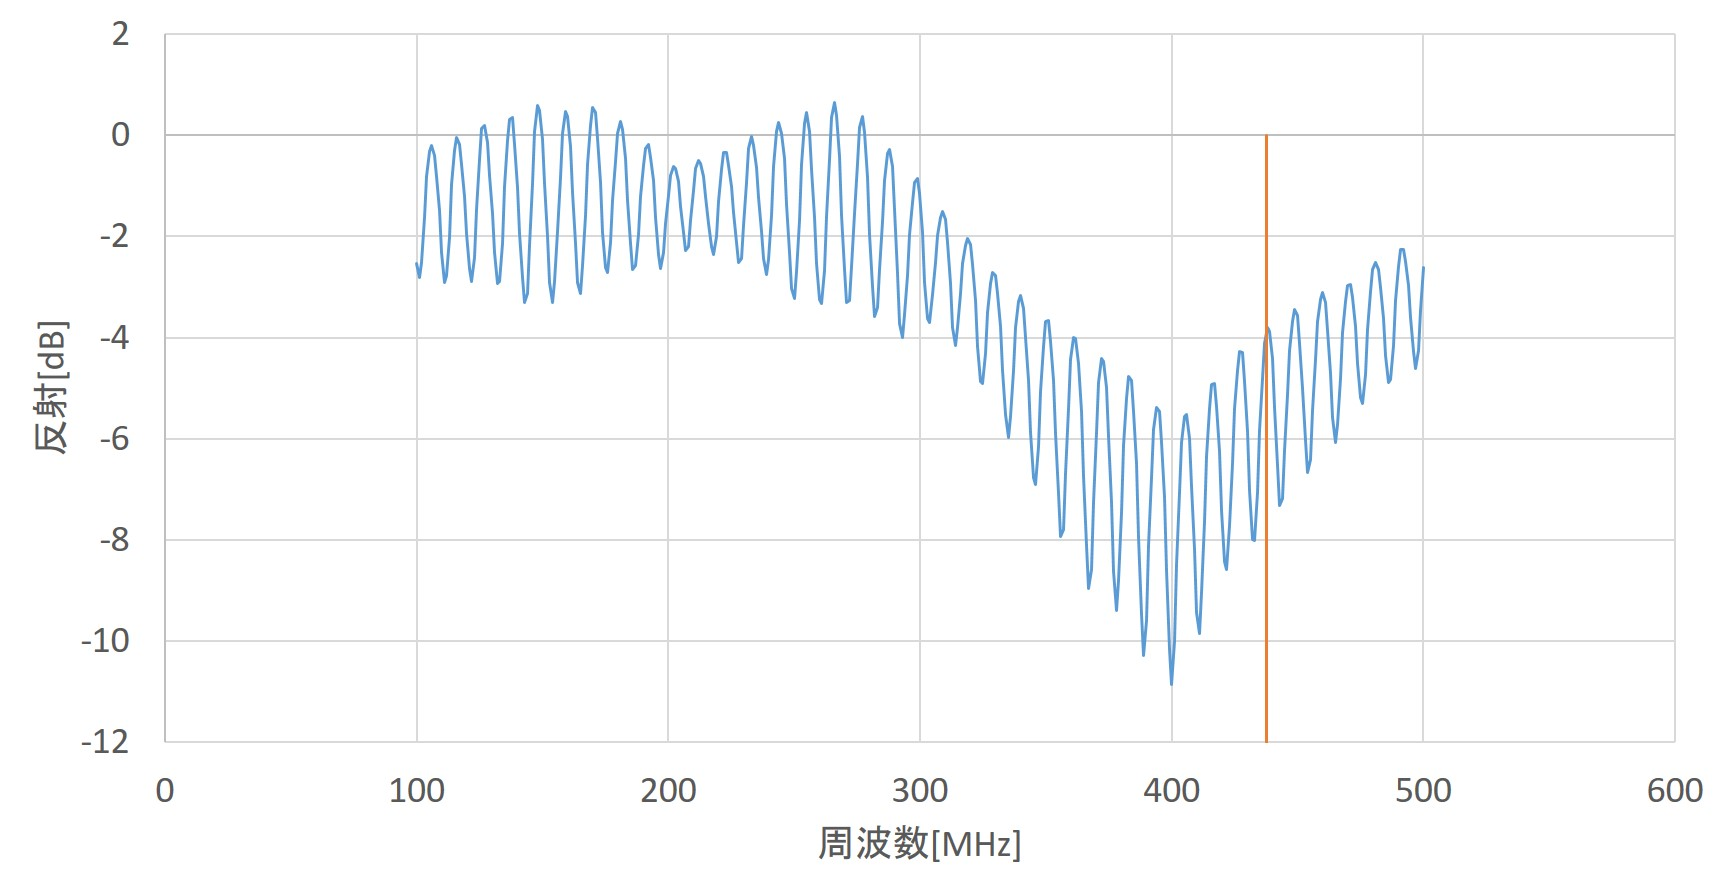
\includegraphics[scale=0.5]{04/fig/4-7-3-2.jpg}
		\caption{FMモノポールアンテナ反射計測結果(VHF)}
		\label{fig4-7-3-2}
	\end{figure}
	

\end{enumerate}

\subsection{モノポールアンテナ 放射特性試験}
本試験ではモノポールアンテナの指向性特性を測定し,健全な指向性を有していることを確認するために行った.
計測結果を図\ref{fig4-7-4}-\ref{fig4-7-4-2}に示す.
ここでもそもそも水平面,垂直面ともに計測するべきであるが,水平面しか計測していない.このようなことを避けるためにしっかりと勉強しましょう.

\begin{figure}[H]
	\centering
	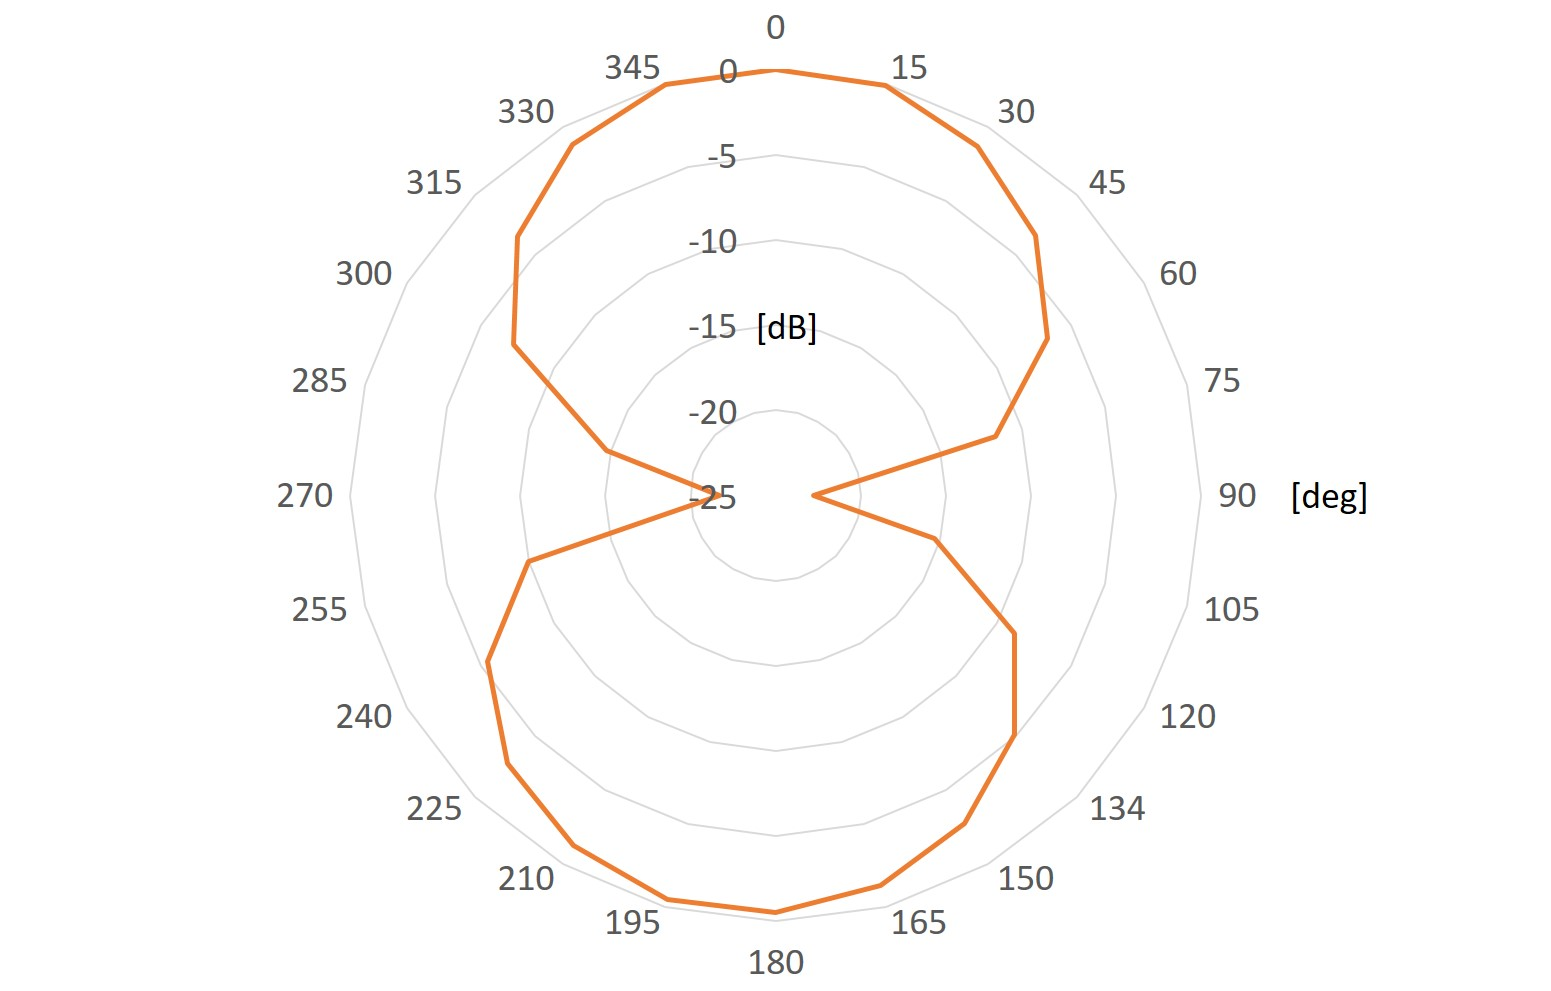
\includegraphics[scale=0.5]{04/fig/4-7-4.jpg}
	\caption{FMモノポールアンテナH-plane放射特性(VHF)}
	\label{fig4-7-4}
\end{figure}
\begin{figure}[H]
	\centering
	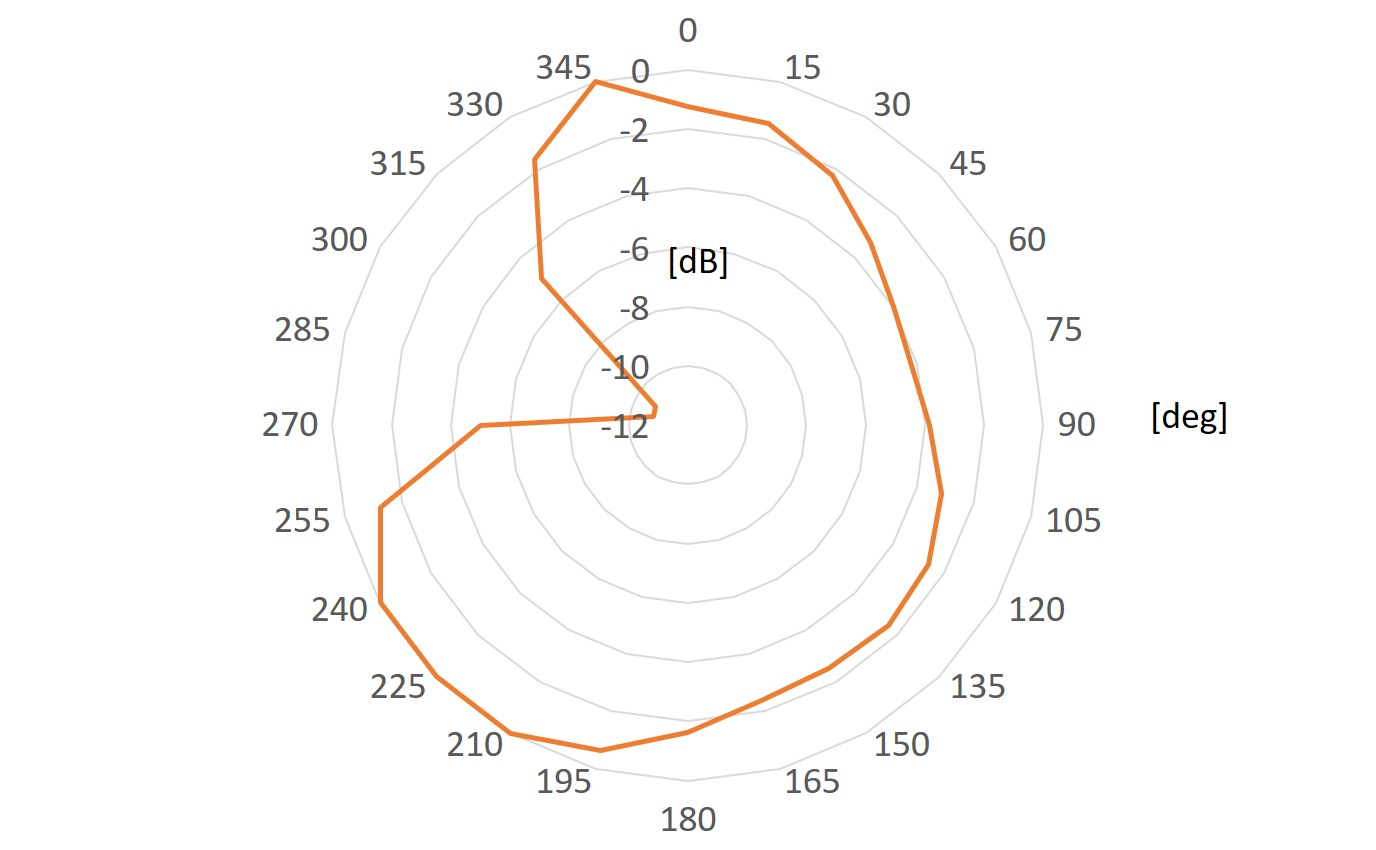
\includegraphics[scale=0.5]{04/fig/4-7-4-2.jpg}
	\caption{FMモノポールアンテナH-plane放射特性(UHF)}
	\label{fig4-7-4-2}
\end{figure}

\subsection{パッチアンテナ 利得・放射特性試験}
本試験ではパッチアンテナの利得,軸比,指向性特性を測定し,所望の性能を有していることを確認するために行った.

\begin{figure}[H]
	\centering
	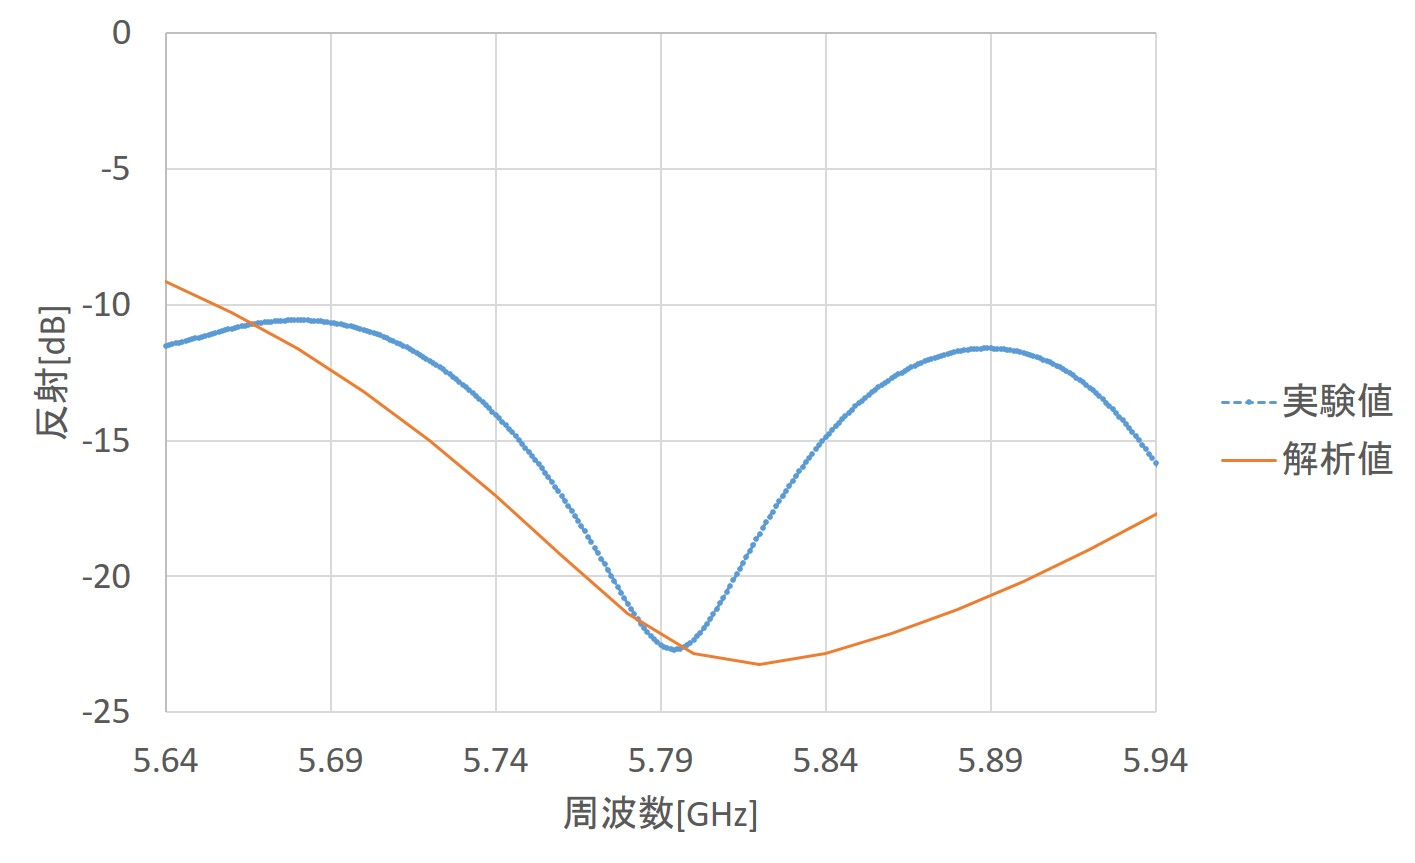
\includegraphics[scale=0.5]{04/fig/4-7-5.jpg}
	\caption{FMパッチアンテナ反射特性}
	\label{fig4-7-5}
\end{figure}
\begin{figure}[H]
	\centering
	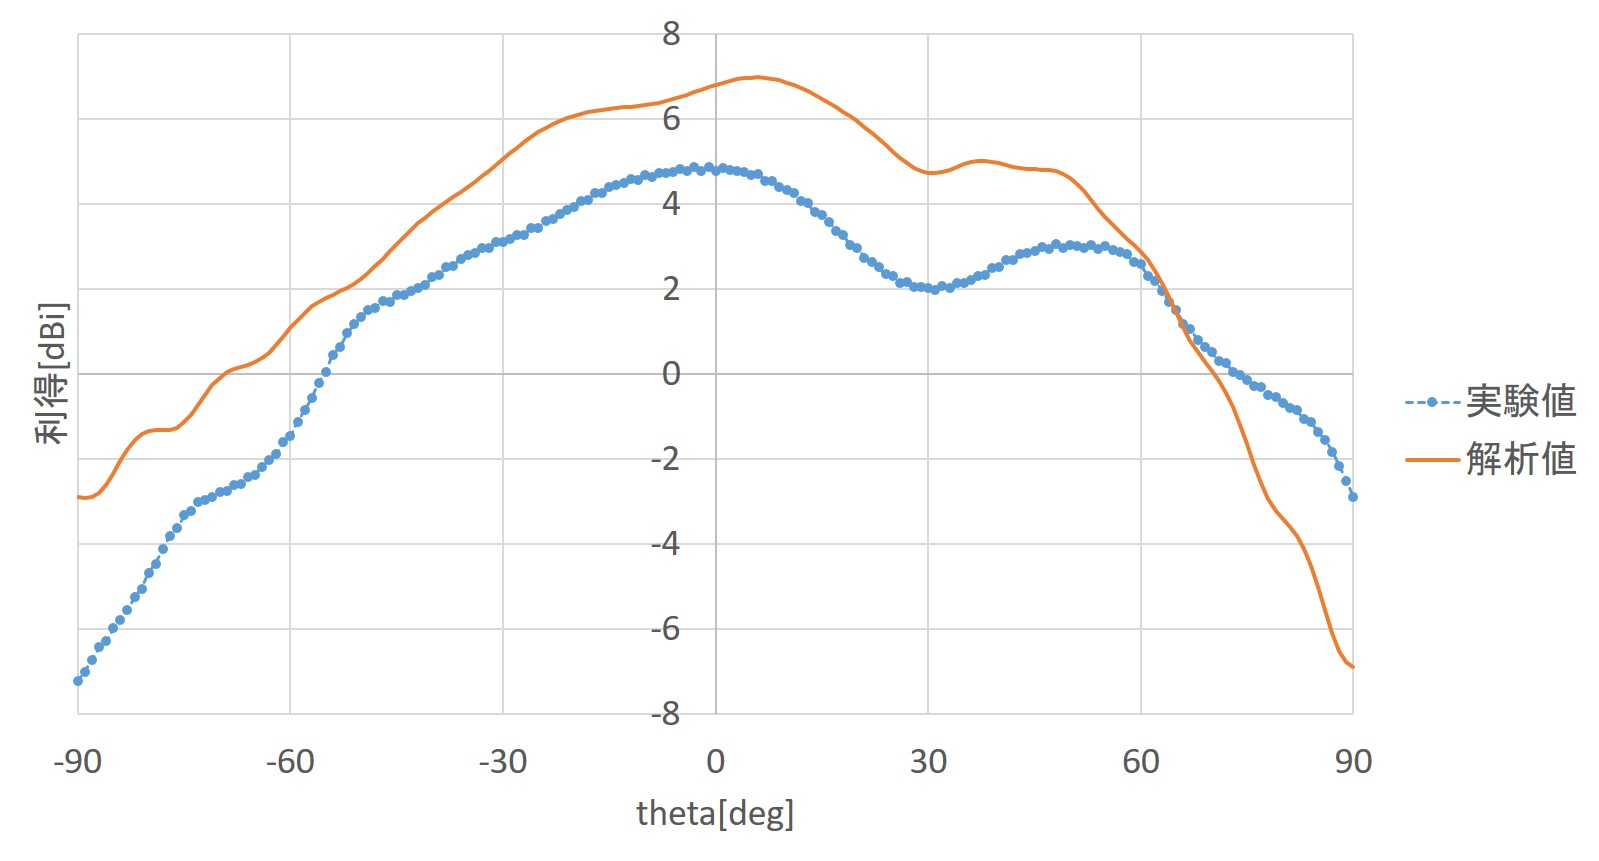
\includegraphics[scale=0.5]{04/fig/4-7-6.jpg}
	\caption{FMパッチアンテナ放射特性}
	\label{fig4-7-6}
\end{figure}
\begin{figure}[H]
	\centering
	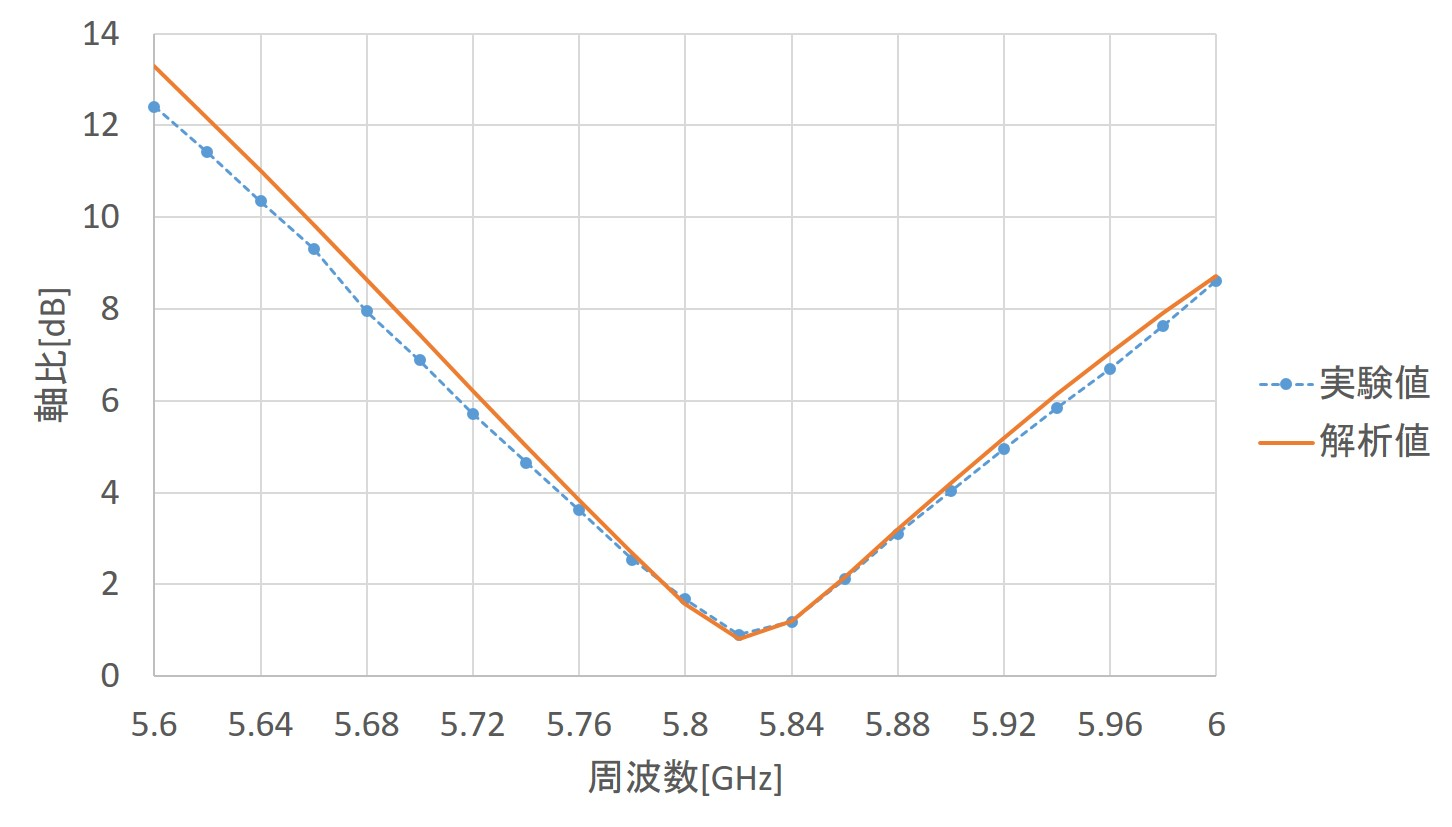
\includegraphics[scale=0.5]{04/fig/4-7-7.jpg}
	\caption{FMパッチアンテナ軸比}
	\label{fig4-7-7}
\end{figure}

\subsection{長距離通信模擬試験}
本試験では,東工大屋上に通信機を設置し,不要電波を漏らさないように適切なアッテネータを取り付けた状態で電波を送信,地上局での受信確認を行うことによって,モノポールアンテナの健全性,東工大地上局設備の健全性を確認することを目的として行った.アンテナの性能は電波暗室試験で計測しており,理屈ではこの試験は必要ないものであるが,気持ちの問題で実施した.

\subsection{反省点}
本衛星の開発でアンテナの特性計測を始めたのは2017年度の12月からであった.
衛星の引き渡しは当初2018年度の夏,伸ばしに伸ばして2018年度の11月であったため明らかにアンテナの特性計測を始めるのが遅かった.
最初のころは訳も分からず,校正など全くしていないVNAを用いてグラウンドでリターンロスの計測などをしていた.
計測に用いる同軸ケーブルも古びたものを用いており,当然ノイズだらけで計測どころではなく,このような試験のために開発メンバーに苦労を掛けてしまったことに申し訳なく感じる.
当初市販品を利用する予定であったパッチアンテナについても同じ時期に特性計測を初めて行い,円偏波ではなく直線偏波になっていることが分かった.
このため,急遽学生でパッチアンテナの設計を行うことになり通信系は非常にドタバタした開発になってしまった.
誰も専門家がいないアンテナという分野について,専門家がいないという危機感が無さ過ぎたように感じる.
後継機の開発などを行う際は設計から開発まで1,,2人程度通信系に集中する人間を用意するべきだった.

